\documentclass{report}

%                       MAIN PACKAGES                       %
% --------------------------------------------------------- %

\usepackage[english]{babel}
\usepackage{graphicx}
\usepackage{caption}
\usepackage{isolatin1}
\usepackage{amssymb}
\usepackage{textcomp}
\usepackage[usenames,dvipsnames]{color}
\usepackage{soul}
\usepackage{cancel}
\usepackage{booktabs}
\usepackage{multirow}
\usepackage{framed}
\usepackage[table]{xcolor}
\usepackage{algpseudocode}
\usepackage[linesnumbered]{algorithm2e} % for psuedo code
\usepackage{courier}
\usepackage{mathtools} % loads amsmath
\usepackage{forest}
\usepackage{tikz}
\usepackage{tikz-qtree}
\usepackage{interval}
\usetikzlibrary{positioning,decorations.pathreplacing}
\usetikzlibrary{calc}

%                         MARGINS                           %
% --------------------------------------------------------- %

\hoffset=-0.5in
\voffset=-0.6in
\oddsidemargin=0pt
\topmargin=0pt
\headheight=12pt
\headsep=15pt
\textheight=690pt
\textwidth=543pt
\marginparsep=11pt
\marginparwidth=54pt
\footskip=25pt
\marginparpush=5pt
\paperwidth=597pt
\paperheight=845pt

%                        PAGE STYLE                         %
% --------------------------------------------------------- %

\usepackage{fancyhdr}
\pagestyle{fancy}
\lhead{CLRS {--} Chapter 8 {--} Sorting in Linear Time}
\rhead{Daniel Bastos Moraes}
\cfoot{}
\rfoot{\thepage}
\renewcommand{\headrulewidth}{0.4pt}
\renewcommand{\footrulewidth}{0.4pt}
\newcommand{\Perp}{\perp\! \! \! \perp}


%                       DEFINITIONS                         %
% --------------------------------------------------------- %

\setlength{\parindent}{0cm}

\makeatletter
\renewenvironment{framed}{%
 \def\FrameCommand##1{\hskip\@totalleftmargin
 \fboxsep=\FrameSep\fbox{##1}}%
 \MakeFramed {\advance\hsize-\width
   \@totalleftmargin\z@ \linewidth\hsize
   \@setminipage}}%
 {\par\unskip\endMakeFramed}
\makeatother

\makeatletter
\def\BState{\State\hskip-\ALG@thistlm}
\makeatother

\DeclarePairedDelimiter{\ceil}{\lceil}{\rceil}
\DeclarePairedDelimiter{\floor}{\lfloor}{\rfloor}
\DeclareMathOperator{\Exists}{\exists}
\DeclareMathOperator{\Forall}{\forall}

\def\figuredirectory{images}

\mathchardef\mhyphen="2D % Define a "math hyphen"

\tikzset{every tree node/.style={minimum width=1.95em,draw,circle,font=\footnotesize},
         blank/.style={draw=none},
         edge from parent/.style=
         {draw, edge from parent path={(\tikzparentnode) -- (\tikzchildnode)}},
         level distance=1cm}

\DeclareMathOperator{\di}{d\!}
\newcommand*\Eval[3]{\left.#1\right\rvert_{#2}^{#3}}

\intervalconfig{soft open fences}

\let\oldnl\nl% Store \nl in \oldnl
\newcommand{\nonl}{\renewcommand{\nl}{\let\nl\oldnl}}% Remove line number for one line

\tikzset{
node of list/.style = {
             draw,
             fill=orange!20,
             minimum height=4.5mm,
             minimum width=4.5mm,
             node distance=6mm
   },
link/.style = {
     -stealth,
     shorten >=1pt
     },
array element/.style = {
    draw, fill=white,
    minimum width = 7mm,
    minimum height = 5mm
  }
}

\def\LinkedList#1{%
  \foreach \index/\element in \list {
     \node[node of list, right = of aux, name=\index] {\element};
     \node[node of list, name=aux2, anchor=west] at ([xshift=-.4pt] \index.east) {};
     \draw[link] (aux) -- (\index);
     \coordinate (aux) at (aux2);
   }
   \fill (aux) circle(2pt);
}

%                        DOCUMENT                           %
% --------------------------------------------------------- %

\begin{document}

\small

{\large Section 8.1 {--} Lower bounds for sorting}

\begin{enumerate}

\item[8.1{-}1]{What is the smallest possible depth of a leaf in a decision tree
for a comparison sort?}

\begin{framed}
The smallest possible depth of a leaf in a decision tree
can be obtained by calculating the shortest simple path from the root to any
of its reachable leaves. This smallest path occurs when the comparisons is made
in the sorted order. For instance, if the input array is sorted, the following
comparisons suffices
\begin{equation*}
\begin{aligned}
  a_1 &\le a_2,\\
  a_2 &\le a_3,\\
  &\;\;\vdots\\
  a_{n - 1} &\le a{n}.
\end{aligned}
\end{equation*}

Thus, the smallest depth of a leaf is any decision tree is $n - 1 = \Theta(n)$.

\end{framed}

\item[8.1{-}2]{Obtain asymptotically tight bounds on $\lg(n!)$ without using
Stirling's approximation. Instead, evaluate the summation $\sum_{k = 1}^n \lg k$
using techniques from Section A.2.}

\begin{framed}
Assume for convenience that $n$ is even. For a lower bound, we have
\begin{equation*}
\begin{aligned}
  \lg{n!} &=   \lg(n \cdot (n - 1) \cdot (n - 2) \cdots 1)\\
          &=   \sum_{k = 1}^{n} \lg k\\
          &=   \sum_{k = 1}^{n/2} \lg k + \sum_{k = n/2 + 1}^{n} \lg k\\
          &\ge \sum_{k = 1}^{n/2} 0 + \sum_{k = n/2 + 1}^{n} \lg (n/2)\\
          &=   \frac{n}{2} \lg{\frac{n}{2}}\\
          &=   \frac{n}{2} \lg n - \frac{n}{2}\\
          &=   \Omega(n \lg n).
\end{aligned}
\end{equation*}

And for an upper bound, we have
\begin{equation*}
\begin{aligned}
  \lg{n!} &=   \lg(n \cdot (n - 1) \cdot (n - 2) \cdots 1)\\
          &=   \sum_{k = 1}^{n} \lg k\\
          &\le \sum_{k = 1}^{n} \lg n\\
          &=   O(n \lg n).
\end{aligned}
\end{equation*}

Thus, $\lg n! = \Theta(n \lg n)$.
\end{framed}

\newpage

\item[8.1{-}3]{Show that there is no comparison sort whose running time is
linear for at least half of the $n!$ inputs of length $n$. What about a fraction
of $1/n$ of the inputs of length $n$?  What about a fraction $1/2^n$?}

\begin{framed}
Such algorithm only exists if we can build a decision tree such that at least
$n!/2$ of its $n!$ leaves has a depth of $\Theta(n)$. Suppose this decision tree
exists. Let $m$ be the depth of the leaf with the ($n!/2$)th smallest depth.
Remove all nodes with depth greater than $m$. The result is a decision tree
with height $m$ and at least $n!/2$ leaves. Using the same reasoning as in the
proof of Theorem 8.1, for every decision tree with at least $n!/2$ leaves, we
have
\[
  \frac{n!}{2} \le l \le 2^{m},
\]
which implies
\[
  m \ge \lg \frac{n!}{2} = \lg n! - 1 = \Omega(n \lg n),
\]
which proves that such a decision tree does not exists. The same reasoning can
be applied to obtain the maximum depth of any fraction of the inputs. For
a fraction of $1/n$, we have
\[
  m \ge \lg \frac{n!}{n} = \lg n! - \lg n = \Omega(n \lg n),
\]
and for a fraction of $1/2^n$, we have
\[
  m \ge \lg \frac{n!}{2^n} = \lg n! - \lg 2^n = \lg n! - n = \Omega(n \lg n).
\]
\end{framed}

\item[8.1{-}4]{Suppose that you are given a sequence of $n$ elements to sort.
The input sequence consists of $n/k$ subsequences, each containing $k$ elements.
The elements in a given subsequence are all smaller than the elements in the
succeeding subsequence and larger than the elements in the preceding
subsequence. Thus, all that is needed to sort the whole sequence of length
$n$ is to sort the $k$ elements in each of the $n/k$ subsequences. Show an
$\Omega(n \lg k)$ lower bound on the number of comparisons needed to solve this
variant of the sorting problem. (\emph{Hint}: It is not rigorous to simply
combine the lower bounds for the individual subsequences.)}

\begin{framed}
All we know is the ordering of the elements of a given subsequence with respect
to the elements of the previous/next subsequence. Thus, for each subsequence,
we have $k!$ possible permutations. Since there are $n/k$ input subsequences,
the number of possible outcomes for this sorting problem is
\[
  \prod_{i = 1}^{n/k} k! = k!^{(n/k)}.
\]

We can use here the same argument used in the text book to prove a lower bound
for any comparison sort algorithm. However, in this case, the number of possible
permutations is $k!^{(n/k)}$, instead of $n!$.  Thus, we need to show that the
height of any decision tree with at least $k!^{(n/k)}$ leaves is
$\Omega(n \lg k)$.  We have
\[
  k!^{n/k} \le l \le 2^h,
\]
which implies
\begin{equation*}
\begin{aligned}
h &\ge \lg \left( k!^{(n/k)} \right)\\
  &=   \frac{n}{k} \cdot \lg k!\\
  &=   \frac{n}{k} \cdot \sum_{i = 1}^{k} \lg i\\
  &=   \frac{n}{k} \cdot \sum_{i = 1}^{\floor{k/2}} \lg i + \frac{n}{k} \cdot \sum_{i = \floor{k/2} + 1}^{k} \lg i\\
  &\ge \frac{n}{k} \cdot \sum_{i = \floor{k/2}}^{k} \lg i\\
  &\ge \frac{n}{k} \cdot \left( \frac{k}{2} \lg \frac{k}{2} \right)\\
  &=   \frac{n}{2} \lg \frac{k}{2}\\
  &=   \Omega(n \lg k).\\
\end{aligned}
\end{equation*}
\end{framed}

\end{enumerate}

\newpage

{\large Section 8.2 {--} Counting sort}

\begin{enumerate}

\item[8.2-1]{Using Figure 8.2 as a model, illustrate the operation of
\textsc{Counting-Sort} on the array
$A = \langle 6, 0, 2, 0, 1, 3, 4, 6, 1, 3, 2 \rangle$.}

\begin{framed}
\newcommand\x{${--}$}
\newcommand\y{\cellcolor{white}}
\newcommand\z{\rowcolor{gray!15}}
\[
\begin{array}{cccccccccccc c cccccccc}
  \y   & 1  & 2  & 3  & 4  & 5  & 6  & 7  & 8  & 9  & 10 & 11 & \y &
  \y   & 0  & 1  & 2  & 3  & 4  & 5  & 6\\
  \z
  \y A & 6  & 0  & 2  & 0  & 1  & 3  & 4  & 6  & 1  & 3  & 2  & \y &
  \y C & 2  & 2  & 2  & 2  & 1  & 0  & 2\\\\
  \z
  \y   & \y & \y & \y & \y & \y & \y & \y & \y & \y & \y & \y & \y &
  \y C & 2  & 4  & 6  & 8  & 9  & 9  & 11\\\\
  \z
  \y B & \x & \x & \x & \x & \x & 2  & \x & \x & \x & \x & \x & \y &
  \y C & 2  & 4  & 5  & 8  & 9  & 9  & 11\\\\
  \z
  \y B & \x & \x & \x & \x & \x & 2  & \x & 3  & \x & \x & \x & \y &
  \y C & 2  & 4  & 5  & 7  & 9  & 9  & 11\\\\
  \z
  \y B & \x & \x & \x &  1 & \x & 2  & \x & 3  & \x & \x & \x & \y &
  \y C & 2  & 3  & 5  & 7  & 9  & 9  & 11\\\\
  \z
  \y B & \x & \x & \x &  1 & \x & 2  & \x & 3  & 4  & \x & 6  & \y &
  \y C & 2  & 3  & 5  & 7  & 8  & 9  & 10\\\\
  \z
  \y B & \x & \x & \x &  1 & \x & 2  & 3  & 3  & 4  & \x & 6  & \y &
  \y C & 2  & 3  & 5  & 6  & 8  & 9  & 10\\\\
  \z
  \y B & \x & \x & 1  &  1 & \x & 2  & 3  & 3  & 4  & \x & 6  & \y &
  \y C & 2  & 2  & 5  & 6  & 8  & 9  & 10\\\\
  \z
  \y B & \x & 0  & 1  &  1 & \x & 2  & 3  & 3  & 4  & \x & 6  & \y &
  \y C & 1  & 2  & 5  & 6  & 8  & 9  & 10\\\\
  \z
  \y B & \x & 0  & 1  &  1 & 2  & 2  & 3  & 3  & 4  & \x & 6  & \y &
  \y C & 1  & 2  & 4  & 6  & 8  & 9  & 10\\\\
  \z
  \y B & 0  & 0  & 1  &  1 & 2  & 2  & 3  & 3  & 4  & \x & 6  & \y &
  \y C & 0  & 2  & 4  & 6  & 8  & 9  & 10\\\\
  \z
  \y B & 0  & 0  & 1  &  1 & 2  & 2  & 3  & 3  & 4  & 6  & 6  & \y &
  \y C & 0  & 2  & 4  & 6  & 8  & 9  & 9
\end{array}
\]
\end{framed}

\item[8.2-2]{Prove that \textsc{Counting-Sort} is stable.}

\begin{framed}
Suppose that the integer $x$ appears $k$ times in the output array. Since the
\textbf{for} loop of lines 10-12 iterates over the input array backwards, the
first integer $x$ to be added to the output array on line 11 is the rightmost
one. The decrement of the couting of $x$ on line 12 ensures that the next
integer $x$ is added to the output array right before the previous one. This
process repeats $k$ times, until the leftmost integer $x$ is added to the
output array ($k - 1$ positions before the rightmost one). This property ensures
that elements with equal value in the input array appears in the same order in
the output array. Thus, the algorithm is stable.
\end{framed}

\item[8.2-3]{Suppose that we were to rewrite the \textbf{for} loop header in
line 10 of the \textsc{Counting-Sort} as

$10\quad\text{\textbf{for}}\;j = 1\;\text{\textbf{to}}\;A.length$

Show that the algorithm still works properly. Is the modified algorithm stable?
}

\begin{framed}
The only difference will be in the \textbf{for} loop of lines 10-12, in which
elements with equal value in the input array will now be added to the output
array in the same order as they appear in the input array. As observed on
Question 8.2-2, each time an element with value $x$ is added to the output
array, the next element with value $x$ is added right before the previous one.
This implies that elements with equal value in the input array will appear in
reverse order in the output array. Thus, this modified algorithm is not stable.
\end{framed}

\item[8.2-4]{Describe an algorithm that, given $n$ integers in the range $0$ to
$k$, preprocesses its input and then answers any query about how many of the $n$
integers fall into a range $[a \dots b]$ in $O(1)$ time. Your algorithm should
use $\Theta(n + k)$ preprocessing time.}

\begin{framed}
For the preprocessing phase, build the array $C$ in the same way it is built in
the \textsc{Couting-Sort} procedure (lines 1-8). This preprocessing will run in
$\Theta(k) + \Theta(n) + \Theta(k) = \Theta(n + k)$. If $a > 0$, answer
$C[b] - C[a - 1]$. Otherwise, answer $C[b]$.
\end{framed}

\end{enumerate}

\newpage

{\large Section 8.3 {--} Radix sort}

\begin{enumerate}

\item[8.3-1]{Using Figure 8.3 as a model, illustrate the operation of
\textsc{Radix-Sort} on the following list of English words: COW, DOG, SEA, RUG,
ROW, MOB, BOX, TAB, BAR, EAR, TAR, DIG, BIG, TEA, NOW, FOX.}

\begin{framed}
\newcommand{\x}[1]{\textbf{#1}}
\begin{center}
\texttt{
\begin{tabular}{c}
  COW\\
  DOG\\
  SEA\\
  RUG\\
  ROW\\
  MOB\\
  BOX\\
  TAB\\
  BAR\\
  EAR\\
  TAR\\
  DIG\\
  BIG\\
  TEA\\
  NOW\\
  FOX
\end{tabular}
}
$\rightarrow$
\texttt{
\begin{tabular}{c}
  SE\x{A}\\
  TE\x{A}\\
  MO\x{B}\\
  TA\x{B}\\
  DO\x{G}\\
  RU\x{G}\\
  DI\x{G}\\
  BI\x{G}\\
  BA\x{R}\\
  EA\x{R}\\
  TA\x{R}\\
  CO\x{W}\\
  RO\x{W}\\
  NO\x{W}\\
  BO\x{X}\\
  FO\x{X}
\end{tabular}
}
$\rightarrow$
\texttt{
\begin{tabular}{c}
  T\x{A}B\\
  B\x{A}R\\
  E\x{A}R\\
  T\x{A}R\\
  S\x{E}A\\
  T\x{E}A\\
  D\x{I}G\\
  B\x{I}G\\
  M\x{O}B\\
  D\x{O}G\\
  C\x{O}W\\
  R\x{O}W\\
  N\x{O}W\\
  B\x{O}X\\
  F\x{O}X\\
  R\x{U}G
\end{tabular}
}
$\rightarrow$
\texttt{
\begin{tabular}{c}
  \x{B}AR\\
  \x{B}IG\\
  \x{B}OX\\
  \x{C}OW\\
  \x{D}IG\\
  \x{D}OG\\
  \x{E}AR\\
  \x{F}OX\\
  \x{M}OB\\
  \x{N}OW\\
  \x{R}OW\\
  \x{R}UG\\
  \x{T}AB\\
  \x{T}AR\\
  \x{T}EA\\
  \x{S}EA
\end{tabular}
}
\end{center}
\end{framed}

\item[8.3-2]{Which of the following sorting algorithms are stable: insertion
sort, merge sort, heapsort, and quicksort? Give a simple scheme that makes any
comparison sort stable. How much additional time and space does your scheme
entail?}

\begin{framed}
\textsc{Insertion-Sort} and \textsc{Merge-Sort} are stable. \textsc{Heapsort}
and \textsc{Quicksort} are not. To make any sorting algorithm stable, we can
store the original index of each element in the array and use this index to
break ties. The additional space required is $\Theta(n)$. The asymptotic running
time is the same, since the number of comparisons will be at most twice.
\end{framed}

\item[8.3-3]{Use induction to prove that radix sort works. Where does your proof
need the assumption that the intermediate sort is stable?}

\begin{framed}
Let $d$ be the number of columns in the input array, where the $d$th column
contains the highest-order digit. \textsc{Radix-Sort} sorts one column at
a time, from the column with the lowest-order digits to the column with the
highest-order digits. The base case occurs when $d = 1$. Since in this case the
elements on the array has a single digit, calling \textsc{Radix-Sort} in this
case is the same as calling its sorting subroutine directly with the input array
as an argument. Thus, \textsc{Radix-Sort} is correct when $d = 1$. Now assume
\textsc{Radix-Sort} works for $d - 1$ columns. Note that sorting $d$ columns is
equivalent to sorting $d - 1$ columns followed by calling the sorting subroutine
on the $d$th column. The induction hypothesis ensures that \textsc{Radix-Sort}
sorts $d - 1$ columns correctly. Since the sorting subroutine is stable, when
sorting the $d$th column, digits that have the same value in the $d$th column
will be kept in the same order as it was after sorting the $(d - 1)$th column.
This implies that \textsc{Radix-Sort} breaks ties on higher-order digits by the
lower-order digits, which is correct.

The sorting subroutine must be stable since a tie that occur while sorting the
$i$th digit is determined by the previous sorts of the lower-order digits. Since
lower-order digits are sorted before higher-order digits, this property is
ensured with an stable sorting algorithm.
\end{framed}

\item[8.3-4]{Show how to sort $n$ integers in the range $0$ to $n^3 - 1$ in
$O(n)$ time.}

\begin{framed}
An integer in the range $0$ to $n^3 - 1$ is represented with at most
$\lg n^3 = 3 \lg n$ bits. We can view a $(3 \lg n)$-bit integer as three
$(\lg n)$-bit integers, so that $b = 3 \lg n$ and $r = \lg n$. With these
settings, \textsc{Radix-Sort} correctly sorts these numbers in
\[
  \Theta\left( \frac{b}{r} \left( n + 2^r \right) \right)
  = \Theta\left( \frac{3 \lg n}{\lg n} \left(n + 2^{\lg n}\right) \right)
  = \Theta( 3 (n + n) )
  = \Theta(n).
\]
\end{framed}

\newpage

\item[8.3-5]{($\star$) In the first card-sorting algorithm in this section,
exactly how many sorting passes are needed to sort $d$-digit decimal numbers in
the worst case? How many piles of cards would an operator need to keep track of
in the worst case?}

\begin{framed}
Suppose that the card-sorting machine represents numbers in base $p$, such
that $2 \le p \le 10$. For a given value of $p$, we have
\begin{itemize}
  \item Each card uses $c = \ceil{\log_p 10^d}$ columns;
  \item Each column uses up to $p$ places.
\end{itemize}

Let $c$th-digit denote the most significant digit, the $(c - 1)$th-digit
denote the 2nd most significant digit, and so on.

The algorithm is recursive. It starts sorting on the $c$th-digit, which
requires $p$ piles to distribute the cards in the worst-case. In the next level,
the algorithm sorts each of the $p$ piles on the $(c - 1)$th-digit, which
requires $p^2$ piles to distribute the cards in the worst-case (each of the
$p$ piles is splitted into $p$ piles). This process goes for $c$ levels. Since
the piles of the previous level can be reutilized in the current level, the
number of piles required to distribute the cards in all levels is the number of
piles required in the last level, which is
\[
  p^c.
\]

Note that to sort the cards on the $c$th-digit, only one sorting pass is needed
to distribute the cards into $p$ piles. To sort on the next digit, these $p$
piles that were sorted on the $c$th-digit must now be sorted on the
$(c - 1)$th-digit, which will require another $p^1$ sorting passes to distribute
them into $p^2$ piles. In general, to sort on the $i$th digit, $p^{c - i}$
sorting passes are required in the worst-case. Thus, the number of sorting
passes in the worst-case is
\[
  \sum_{i = 1}^{c} p^{c - i} = \sum_{i = 0}^{c - 1} p^{i} = \frac{p^c - 1}{p - 1}.
\]

\end{framed}

\end{enumerate}

\newpage

{\large Section 8.4 {--} Bucket sort}

\begin{enumerate}

\item[8.4-1]{Using Figure 8.4 as a model, illustrate the operation of
\textsc{Bucket-Sort} on the array
$A = \langle .79, .13, .16, .64, .39, .20, .89, .53, .71, .42 \rangle$.}

\begin{framed}
\begin{center}
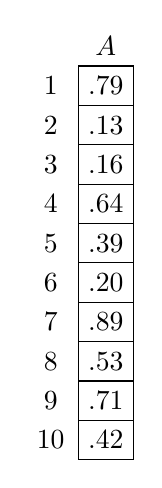
\begin{tikzpicture}
\node at (0, 0) {$A$};
\foreach \index/\element/\list in {1/.79, 2/.13, 3/.16, 4/.64, 5/.39, 6/.20,
                                   7/.89, 8/.53, 9/.71, 10/.42} {
   \node[array element] (aux) at (0,-\index/2) {\element};
   \node at (-0.7, -\index/2) {\index};
}
\end{tikzpicture}
\qquad
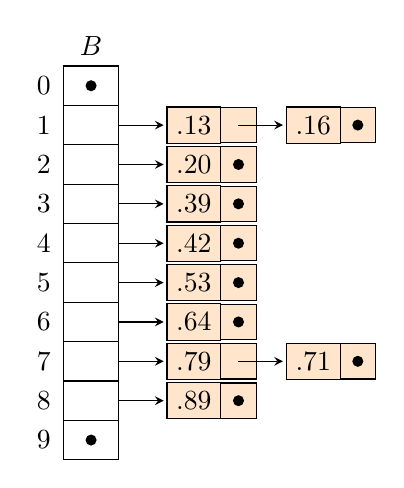
\begin{tikzpicture}
\node at (0, 0.5) {$B$};
  \foreach \index/\list in {0/, 1/{1/.13, 2/.16}, 2/{1/.20}, 3/{1/.39},
                            4/{1/.42}, 5/{1/.53}, 6/{1/.64}, 7/{1/.79, 2/.71},
                            8/{1/.89}, 9/} {
   \node[array element] (aux) at (0,-\index/2) {};
   \node at (-0.6, -\index/2) {\index};
   \LinkedList{\list}
}
\end{tikzpicture}
\end{center}
\end{framed}

\item[8.4-2]{Explain why the worst-case running time for bucket sort is
$\Theta(n^2)$. What simple change to the algorithm preserves its linear
average-case running time and makes its worst-case running time $O(n \lg n)$?}

\begin{framed}
The worst-case occurs when the input array is in decreasing order and every
element falls into the same bucket. Since \textsc{Insertion-Sort} takes
$\Theta(n^2)$ to sort an array of size $n$ that is in decreasing order, bucket
sort will run in $\Theta(n^2)$.

The worst-case running time can be improved replacing \textsc{Insertion-Sort}
with $\textsc{Heapsort}$, which will make it run in $O(n \lg n)$. As for the
average-case, the expected running time of this variation of bucket sort is
\begin{equation*}
\begin{aligned}
  \text{E}[T(n)] &= \text{E}\left[ \Theta(n) + \sum_{i = 0}^{n - 1} O(n_i \lg n_i) \right]\\
                 &= \Theta(n) + \sum_{i = 0}^{n - 1} \text{E}[O(n_i \lg n_i)]\\
                 &= \Theta(n) + \sum_{i = 0}^{n - 1} O(\text{E}[n_i \lg n_i]).
\end{aligned}
\end{equation*}

Using the same logic adopted in the text book to compute $\text{E}[n_i^2]$, we
have
\[
  n_i = \sum_{j = 1}^{n} X_{ij},
\]
which implies
\begin{equation*}
\begin{aligned}
  \text{E}[n_i \lg n_i] &=   \text{E}\left[ \sum_{j = 1}^{n} X_{ij} \lg \sum_{j = 1}^{n} X_{ij} \right]\\
                        &\le \text{E}\left[ \sum_{j = 1}^{n} X_{ij} \sum_{j = 1}^{n} X_{ij} \right]\\
                        &=   2 - \frac{1}{n}. & \text{(from equation (8.2))}
\end{aligned}
\end{equation*}

Thus, the average-case running time of this variation of bucket sort is
\[
  \text{E}[T(n)] = \Theta(n) + \sum_{i = 0}^{n - 1} O\left(2 - \frac{1}{n}\right)
                 = \Theta(n) + n \cdot O\left(1\right)
                 = \Theta(n).
\]
\end{framed}

\newpage

\item[8.4-3]{Let $X$ be a random variable that is equal to the number of heads
in two flips of a fair coin. What is $\text{E}[X^2]$? What is $\text{E}^2[X]$?}

\begin{framed}
Lets define the indicator random variable
\[
  X_i = \text{I}\{\text{flip } i \text{ comes up heap}\}.
\]

Thus, we have
\[
  X = X_1 + X_2,
\]
and
\[
  X^2 = (X_1 + X_2)^2 = X_1^2 + 2 X_1 X_2 + X_2^2.
\]

Note that
\[
  \text{E}[X_i] = \text{Pr}\{X_i = 1\} = \frac{1}{2},
\]
and
\[
  \text{E}[X_i^2] = 1^2 \cdot \frac{1}{2} + 0^2 \cdot \frac{1}{2} = \frac{1}{2}.
\]

Using the above definitions and linearity of expectation, we have
\begin{equation*}
\begin{aligned}
  \text{E}[X^2] &= \text{E}[X_1^2 + 2 X_1 X_2 + X_2^2]\\
                &= \text{E}[X_1^2] + 2 \text{E}[X_1 X_2] + \text{E}[X_2^2]\\
                &= \frac{1}{2} + 2 \left(\text{E}[X_1] \text{E}[X_2]\right) + \frac{1}{2} & \text{(since $X_1$ and $X_2$ are independent)}\\
                &= \frac{1}{2} + 2 \left(\frac{1}{2} \cdot \frac{1}{2}\right) + \frac{1}{2}\\
                &= \frac{3}{2},
\end{aligned}
\end{equation*}
and
\begin{equation*}
\begin{aligned}
  \text{E}^2[X] &= \text{E}^2[X_1 + X_2]\\
                &= \text{E}[X_1 + X_2] \text{E}[X_1 + X_2]\\
                &= ( \text{E}[X_1] + \text{E}[X_2] ) ( \text{E}[X_1] + \text{E}[X_2] )\\
                &= \left( \frac{1}{2} + \frac{1}{2} \right) \left( \frac{1}{2} + \frac{1}{2} \right)\\
                &= 1.
\end{aligned}
\end{equation*}
\end{framed}

\newpage

\item[8.4-4]{($\star$) We are given $n$ points in the unit circle,
$p_i = (x_i, y_i)$, such that $0 < x^2_i + y^2_i \le 1$ for
$i = 1, 2, \dots, n$. Suppose that the points are uniformly distributed; that
is, the probability of finding a point in any region of the circle is
proportional to the area of that region. Design an algorithm with an
average-case running time of $\Theta(n)$ to sort the $n$ points by their
distances $d_i = \sqrt{x^2_i + y^2_i}$ from the origin. (\emph{Hint:} Design the
bucket sizes in \textsc{Bucket-Sort} to reflect the uniform distribution of the
points in the unit circle.)}

\begin{framed}

Considering that the points are uniformly distributed over the area of the unit
circle, we can divide the circle into $n$ rings with equal area, such that the
expected number of points in each ring is $1$. The figure below illustrates
a circle that is divided into three rings with equal area.

\begin{center}
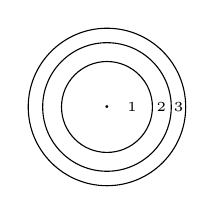
\begin{tikzpicture}[black]
  \draw node at (0.0, 0.0) {.};
  \draw node at (0.32, 0.0) {\tiny 1};
  \draw node at (0.69, 0.0) {\tiny 2};
  \draw node at (0.91, 0.0) {\tiny 3};
  \foreach \i in {1, 2, 3} {
    \draw (0,0) circle ({sqrt(\i) / sqrt(3)});
  }
\end{tikzpicture}
\end{center}

We them assign to the $i$th bucket the points that falls within the $i$th ring,
sort each bucket individually with \textsc{Insertion-Sort}, and combine the
elements of each bucket sequentially. This is basically the \textsc{Bucket-Sort}
algorithm with a modification on the way we assign the elements to the buckets.
Since the distribution of points over the buckets is uniform, the average-case
running time of this algorithm is still $O(n)$.

We now need a function that maps a point to its bucket. Let $r_i$ denote the
(larger) radius of the $i$th ring. We claim that
\[
  r_i = \frac{\sqrt{i}}{\sqrt{n}},
\]
which implies that a point $p_j$ belongs to the $i$th ring if, and only if,
\[
  \sqrt{\frac{i - 1}{n}} < d_j \le \sqrt{\frac{i}{n}},
\]
squaring both sides and multiplying by $n$, we have
\[
  i - 1 < d_j^2 \cdot n \le i,
\]
which implies
\[
  i = \ceil{d_j^2 \cdot n}.
\]

\textbf{Proof for the radius of the $i$th ring.}

Since the area of the unit circle is $\pi$ and each ring has equal area, for
$i > 0$, we have
\[
  \pi r_i^2 - \pi r_{i - 1}^2 = \frac{\pi}{n},
\]
which implies
\[
  r_i = \sqrt{\frac{1}{n} + r^2_{i - 1}}.
\]

Note that
\begin{equation*}
\begin{aligned}
  r_1 = \sqrt{\frac{1}{n} + 0^2} = \frac{\sqrt{1}}{\sqrt{n}},\\
  r_2 = \sqrt{\frac{1}{n} + \left(\sqrt{\frac{1}{n}}\right)^2} = \frac{\sqrt{2}}{\sqrt{n}},\\
  r_3 = \sqrt{\frac{1}{n} + \left(\sqrt{\frac{2}{n}}\right)^2} = \frac{\sqrt{3}}{\sqrt{n}},
\end{aligned}
\end{equation*}

which lead us to assume that
\[
  r_i = \frac{\sqrt{i}}{\sqrt{n}},
\]
for $i = 0, 1, \dots, n$. We shall prove it by induction. Note that it holds for
$i = 0$, since
\[
  r_0 = \frac{\sqrt{0}}{\sqrt{n}} = 0.
\]
To show that it holds for $i > 0$, we need to show that if it holds for $i$, it
also holds for $i + 1$. We have
\[
  r_{i + 1} = \sqrt{\frac{1}{n} + \left(\sqrt{\frac{i}{n}}\right)^2}
            = \sqrt{\frac{i + 1}{n}}
            = \frac{\sqrt{i + 1}}{\sqrt{n}},
\]
which proves the inductive step.

\end{framed}

\item[8.4-5]{($\star$) A \textbf{\emph{probability distribution function}}
$P(x)$ for a random variable $X$ is defined by $P(x) = \text{Pr}\{X \le x\}$.
Suppose that we draw a list of $n$ random variables $X_1, X_2, \dots, X_n$ from
a continuous probability distribution function $P$ that is computable in $O(1)$
time. Give an algorithm that sorts these numbers in linear average-case time.}

\begin{framed}
Skipped.
\end{framed}

\end{enumerate}

\newpage

{\large Problems}

\begin{enumerate}

\item[8-1]{\textbf{\emph{Probabilistic lower bounds on comparison sorting}}\\
In this problem, we prove a probabilistic $\Omega(n \lg n)$ lower bound on the
running time of any deterministic or randomized comparison sort on $n$ distinct
input elements. We begin by examining a deterministic comparison sort $A$ with
decision tree $T_A$. We assume that every permutation of $A$'s inputs is equally
likely.

\begin{enumerate}
\item[\textbf{a.}]{Suppose that each leaf of $T_A$ is labeled with the
probability that it is reached given a random input. Prove that exactly $n!$
leaves are labeled $1/n!$ and that the rest are labeled 0.}
\item[\textbf{b.}]{Let $D(T)$ denote the external path length of a decision tree
$T$; that is, $D(T)$ is the sum of the depths of all the leaves of $T$. Let $T$
be a decision tree with $k > 1$ leaves, and let $LT$ and $RT$ be the left and
right subtrees of $T$. Show that $D(T) = D(LT) + D(RT) + k$.}
\item[\textbf{c.}]{Let $d(k)$ be the minimum value of $D(T)$ over all decision
trees $T$ with $k > 1$ leaves. Show that
$d(k) = \min_{1 \le i \le k - 1} \{d(i) + d(k - i) + k\}$. (Hint: Consider
a decision tree $T$ with $k$ leaves that achieves the minimum. Let $i_0$ be the
number of leaves in $LT$ and $k - i_0$ the number of leaves in $RT$.)}
\item[\textbf{d.}]{Prove that for a given value of $k > 1$ and $i$ in the range
$1 \le i \le k - 1$, the function $i \lg i + (k - i) \lg (k - i)$ is minimized
at $i = k/2$. Conclude that $d(k) = \Omega(k \lg k)$.}
\item[\textbf{e.}]{Prove that $D(T_A) = \Omega(n! \lg(n!))$, and conclude that
the average-case time to sort $n$ elements is $\Omega(n \lg n)$.}
\end{enumerate}

Now, consider a \emph{randomized} comparison sort $B$. We can extend the
decision-tree model to handle randomization by incorporating two kinds of nodes:
ordinary comparison nodes and ``randomization'' nodes. A randomization node
models a random choice of the form \textsc{Random}$(l, r)$ made by algorithm
$B$; the node has $r$ children, each of which is equally likely to be chosen
during an execution of the algorithm.

\begin{enumerate}
\item[\textbf{f.}]{Show that for any randomized comparison sort $B$, there
exists a deterministic comparison sort $A$ whose expected number of comparisons
is no more than those made by $B$.}
\end{enumerate}
}

\begin{framed}
\begin{enumerate}

\item{First note that there are $n!$ distinct permutations of an input of size
$n$ with distinct elements. To be a valid decision tree, $T_A$ must have each of
these permutations as a reachable leaf. Since every permutation is equally
likely, each of these leaves must be reachable with probability $1/n!$. If $T_A$
has any additional leaf, it is not reachable for any input and has probability
0.}

\item{Note that, since $k > 1$, the root of $T$ if not a leaf. Also, the only
node that is present in $T$ and is not present in the subtrees $LT$ and $RT$
together is the root of $T$. This implies that each leaf at depth $d$ in $T$ is
either in $LT$ or in $RT$, but at depth $d - 1$. Since there are $k$ leaves in
$T$, we have $D(T) = D(LT) + D(RT) + k$.}

\item{
First, we will show that
\[
  d(k) \le \min_{1 \le i \le k - 1} \{d(i) + d(k - i) + k\},
\]
by showing that
\[
  d(k) \le d(i) + d(k - i) + k,
\]
for $i = 1, \dots, k - 1$. For every $i$ such that $1 \le i \le k - 1$, there
exist decision trees $LT$ and $RT$ with $i$ leaves and $k - i$ leaves,
respectivelly, such that $D(LT) = d(i)$ and $D(RT) = d(k - i)$. Let $T$ be
a decision tree composed by a root node and $LT$ and $RT$ as its left and right
subtrees, respectivelly.  Note that $T$ has $k$ leaves, since it has all the
leaves from $LT$ and $RT$, and its root is not a leaf. Then, we have
\begin{equation*}
\begin{aligned}
  d(k) &\le D(T) & \text{(from the definition of $d(\cdot)$)}\\
       &=   D(LT) + D(RT) + k & \text{(from item (b))}\\
       &= d(i) + d(k - i) + k.
\end{aligned}
\end{equation*}

Now, we will show that
\[
  d(k) \ge \min_{1 \le i \le k - 1} \{d(i) + d(k - i) + k\},
\]
by showing that
\[
  \Exists i \in 1, \dots, k - 1 \; | \; d(k) \ge d(i) + d(k - i) + k.
\]

Let $T$ be a decision tree with $k$ leaves such that $D(T) = d(k)$. Let $LT$ and
$RT$ be the left and right subtrees of $T$ and let $i$ and $k - i$ be the number
of leaves of $LT$ and $RT$, respectivelly. We have
\begin{equation*}
\begin{aligned}
  d(k) &=   D(T) && \text{(from the definition of $T$)}\\
       &=   D(LT) + D(RT) + k && \text{(from item (b))}\\
       &\ge d(i) + d(k - i) + k.
\end{aligned}
\end{equation*}

Then, we can conclude that
\[
  d(k) = \min_{1 \le i \le k - 1} \{d(i) + d(k - i) + k\}.
\]
}

\newpage

\item{
Let $f(i) = i \lg i + (k - i) \lg (k - i)$. We have
\begin{equation*}
\begin{aligned}
  f'(i) &= \frac{d}{di} \left( i \lg i + (k - i) \lg (k - i) \right)\\
        &= \frac{d}{di} \left( \frac{i \ln i + (k - i) \ln (k - i)}{\ln 2} \right)\\
        &= \frac{d}{di} \left( \frac{i \ln i}{\ln 2} + \frac{(k - i) \ln (k - i)}{\ln 2} \right)\\
        &= \frac{1 + \ln i}{\ln 2} + \frac{- 1 - \ln (k - i)}{\ln 2}\\
        &= \frac{\ln i - \ln (k - i)}{\ln 2}\\
        &= \lg i - \lg (k - i),
\end{aligned}
\end{equation*}
which is 0 when $i = k/2$. Also note that
\[
  f'(1) = f'(k - 1) = \ln(k - 1) \ge \ln 1 = 0 = f(k/2),
\]
which implies that the point $i = k/2$ is a minimum. We shall now prove that
$d(k) = \Omega(k \lg k)$. Our guess is
\[
  d(i) \ge c i \lg i \; \Forall 1 \le i \le k - 1,
\]
where $c$ is a positive constant. Substituting into the recurrence, yields
\begin{equation*}
\begin{aligned}
  d(k) &=   \min_{1 \le i \le k - 1} \{d(i) + d(k - i) + k\}\\
       &\ge \min_{1 \le 1 \le k - 1} \{c (i \lg i + (k - i) \lg (k - i)) + k\}\\
       &=   \min_{1 \le 1 \le k - 1} \{c f(i) + k\}\\
       &=   c f\left(\frac{k}{2}\right) + k\\
       &=   c \left(\frac{k}{2} \lg \frac{k}{2} + \frac{k}{2} \lg \frac{k}{2}\right) + k\\
       &=   c k \lg \frac{k}{2} + k\\
       &=   c k \lg k - c k + k\\
       &\ge c k \lg k,\\
\end{aligned}
\end{equation*}
where the last step holds as long as $c \le 1$.
}

\item{Since $T_A$ has $n!$ leaves, we have
\[
  D(T_A) \ge d(n!) = \Omega(n! \lg n!).
\]

Note that the external path length of a decision tree denotes the number of
comparisons needed to sort every possible permutation of an input of size $n$.
Since each of the $n!$ permutations have the same probability of happening
(from item (a)), the expected number of comparisons for each input is
\begin{equation*}
\begin{aligned}
  \frac{\Omega(n! \lg (n!))}{n!} &= \Omega(\lg (n!))\\
                                 &= \Omega(n \lg n). & \text{(from (3.19))}
\end{aligned}
\end{equation*}
}

\item{Just replace each randomization node with one of its subtrees,
particularly the one with the smaller external path. The result is a valid
deterministic tree with no more comparisons than the radomized tree. Thus, we
can conclude that the number of comparisons for any randomized comparison sort
is also $\Omega(n \lg n)$}.

\end{enumerate}
\end{framed}

\newpage

\item[8-2]{\textbf{\emph{Sorting in place in linear time}}\\
Suppose that we have an array of $n$ data records to sort and that the key of
each record has the value 0 or 1. An algorithm for sorting such a set of records
might possess some subset of the following three desirable characteristics:
\begin{enumerate}
  \item[1.] The algorithm runs in $O(n)$ time.
  \item[2.] The algorithm is stable.
  \item[3.] The algorithm sorts in place, using no more than a constant
    amount of storage space in addition to the original array.
\end{enumerate}

\begin{enumerate}
  \item[\textbf{a.}] Give an algorithm that satisfies criteria 1 and 2 above.
  \item[\textbf{b.}] Give an algorithm that satisfies criteria 1 and 3 above.
  \item[\textbf{c.}] Give an algorithm that satisfies criteria 2 and 3 above.
  \item[\textbf{d.}] Can you use any of your sorting algorithms form parts
    (a)${-}$(c) as the sorting method used in line 2 of \textsc{Radix-Sort}, so
    that \textsc{Radix-Sort} sorts $n$ records with $b$-bit keys in $O(bn)$
    time? Explain how or why not.
  \item[\textbf{e.}] Suppose that the $n$ records have keys in the range from
    1 to $k$. Show how to modify counting sort so that it sorts the records in
    place in $O(n + k)$ time. You may use $O(k)$ storage outside the input
    array. Is your algorithm stable? (\emph{Hint:} How would you do it for $k
    = 3$?)
\end{enumerate}
}

\begin{framed}
\begin{enumerate}
\item{The following is a modified \textsc{Counting-Sort} for data records. If
runs in $\Theta(n)$, is stable, but do not sort in place.

\begin{algorithm}[H]
\SetAlgoNoEnd\DontPrintSemicolon
\BlankLine
\SetKwFunction{algo}{Counting-Sort-Binary-Records}
\SetKwProg{myalg}{}{}{}
\nonl\myalg{\algo{A, B}}{%
  $\text{\emph{one-pos}} = 1$\;
  $\text{\emph{zero-pos}} = 1$\;
  \For{$i = 1$ \KwTo $A.length$}{%
    $\text{\emph{key}} = A[i].\text{\emph{key}}$\;
    \If{$key == 0$}{%
      $\text{\emph{one-pos}} = \text{\emph{one-pos}} + 1$\;
    }
  }
  \For{$i = 1$ \KwTo $A.length$}{%
    $\text{\emph{key}} = A[i].\text{\emph{key}}$\;
    \If{$key == 0$}{%
      $B[\text{\emph{zero-pos}}] = A[i]$\;
      $\text{\emph{zero-pos}} = \text{\emph{zero-pos}} + 1$\;
    }
    \Else{%
      $B[\text{\emph{one-pos}}] = A[i]$\;
      $\text{\emph{one-pos}} = \text{\emph{one-pos}} + 1$\;
    }
  }
}
\end{algorithm}
}

\item{The following uses a technique similar to the one used for the
\textsc{Hoare-Partition}, introduced on Question 7-1. It runs in $\Theta(n)$,
sorts in place, but is not stable.

\begin{algorithm}[H]
\SetAlgoNoEnd\DontPrintSemicolon
\BlankLine
\SetKwFunction{algo}{InPlace-Sort-Binary-Records}
\SetKwProg{myalg}{}{}{}
\nonl\myalg{\algo{A}}{%
  $i = 1$\;
  $j = A.length$\;
  \While{\texttt{\upshape{True}}}{%
    \While{$j > i$ \textbf{\upshape{and}} $A[j].key == 1$}{
      $j = j - 1$\; }
    \While{$i < j$ \textbf{\upshape{and}} $A[i].key == 0$}{%
      $i = i + 1$\; }
    \If{$i < j$}{%
      swap $A[i]$ with $A[j]$\; }
    \Else{%
      break\; } } }
\end{algorithm}
}

\item{The following is a modified \textsc{Insertion-Sort} for data records. It
is stable, sorts in place, but is not linear.

\begin{algorithm}[H]
\SetAlgoNoEnd\DontPrintSemicolon
\BlankLine
\SetKwFunction{algo}{Insertion-Sort-Binary-Records}
\SetKwProg{myalg}{}{}{}
\nonl\myalg{\algo{A}}{%
  \For{$j = 2$ \KwTo $A.length$}{%
    $key = A[j].key$\;
    $i = j - 1$\;
    \While{$i > 0$ \textbf{\upshape{and}} $A[i].key > key$}{%
      $A[i + 1] = A[i]$\;
      $i = i - 1$\; }
    $A[i + 1] = key$\; } }
\end{algorithm}
}

\newpage

\item{To be used as a subroutine of \textsc{Radix-Sort}, the sorting algorithm
must be stable. Also, in order to \textsc{Radix-Sort} run in $O(bn)$ time, the
sorting subroutine must run in $O(n)$. The only algorithm that satisfies both of
these constraints is the one on part (a).}

\item{Roughly speaking, instead of copying each element to its correct position
in a new array, we swap each element with the element that is in its correct
position. The algorithm runs in $\Theta(n + k)$, sorts in place, but is not
stable. The pseudocode is stated below.

\begin{algorithm}[H]
\SetAlgoNoEnd\DontPrintSemicolon
\BlankLine
\SetKwFunction{algo}{Counting-Sort-InPlace}
\SetKwProg{myalg}{}{}{}
\nonl\myalg{\algo{A, k}}{%
  let $C[0, \dots, k]$ be a new array\;
  let $T[0, \dots, k]$ be a new array\;
  \For{$i = 0$ \KwTo $k$}{%
    $C[i] = 0$\; }
  \For{$i = 1$ \KwTo $A.length$}{%
    $key = A[i].key$\;
    $C[key] = C[key] + 1$\; }
  \For{$i = 1$ \KwTo $k$}{%
    $C[i] = C[i] + C[i - 1]$\; }
  \For{$i = 0$ \KwTo $k$}{%
    $T[i] = C[i]$\; }
  $\text{\emph{pos}} = 1$\;
  \While{$\text{pos} < A.length$}{%
    $\text{\emph{key}} = A[pos].\text{\emph{key}}$\;
    \If{$C[\text{key}] > \text{pos}$}{%
      swap $A[\text{\emph{pos}}]$ with $A[C[\text{\emph{key}}]]$\;
      $C[\text{\emph{key}}] = C[\text{\emph{key}}] - 1$\; }
    \Else{%
      $\text{\emph{pos}} = \text{\emph{pos}} + T[\text{\emph{key}}]$\;
    }
  }
}
\end{algorithm}
}

\end{enumerate}
\end{framed}

\newpage

\item[8-3]{\textbf{\emph{Sorting variable-length items}}
\begin{enumerate}
\item[\textbf{a.}]{You are given an array of integers, where different integers
may have different numbers of digits, but the total number of digits over all
the integers in the array is $n$. Show how to sort the array in $O(n)$ time.}
\item[\textbf{b.}]{You are given an array of strings, where different strings
may have different numbers of characters, but the total number of characters
over all the strings is $n$. Show how to sort the strings in $O(n)$ time.
(Note that the desired order here is the standard alphabetical order; for
example, $\texttt{a} < \texttt{ab} < \texttt{b}$.)}
\end{enumerate}
}

\begin{framed}
\begin{enumerate}
\item Let $m$ denote the number of integers in the input array. Start sorting
the numbers by their sign, using an algorithm similar to
\textsc{Counting-Sort-Binary-Records}, in which negative numbers are placed
before positive numbers. This step runs in $O(m)$. Let $m_{pos}$ and $m_{neg}$
denote the number of positive and negative integers, respectivelly. For each
group of numbers with the same sign, sort the elements in the group by their
number of digits with \textsc{Counting-Sort}. This step will take $O(m_{pos}
+ n) + O(m_{neg} + n) = O(n)$. Let $m_i$ denote the number of integers with $i$
digits. For each group of numbers with $i$ digits, sort the elements in the
group with \textsc{Radix-Sort}. Since each call to \textsc{Radix-Sort} runs in
$O(i \cdot (m_i + 10)) = O(i \cdot m_i)$, this step will take
\[
  \sum_{i = 1}^{n} O(i \cdot m_i)
  = O\left( \sum_{i = 1}^{n} (i \cdot m_i) \right)
  = O(n).
\]

Thus, the running time of this algorithm is
\[
  O(m + n + n) = O(n).
\]

\item Note that, different from the problem of sorting integers, we can not use
the length of the string to sort the elements -- strings with longer length does
not imply any order with respect to strings with smaller length. However, the
leftmost character of each string does imply an order. When the first character
of two strings are the same, the strings are untied by their following
character, and so on until the last character. We can use this notion to derive
a recursive algorithm that sorts and groups the strings by their first
character, and recursively sorts each group by their following character.
Note that strings that do not have the current character should be placed before
the ones that does have the character. Since the range of characters is
constant, we can sort each group using counting sort in linear time on the
number of elements in the group. To avoid creating multiple subarrays in each
recursion call, \textsc{Counting-Sort-InPlace} is more suitable.

Let $m$ denote the number of strings in the input array and let $n_i$ denote the
number of characters in the $i$th string. Since counting sort is linear on the
number of elements being sorted and the $i$th string are considered in at most
$n_i + 1$ calls of counting sort (one additional time for the special case when
the string does not have the following character), the total cost of this
algorithm is
\[
  O\left(\sum_{i = 1}^{m} (n_i + 1)\right)
  = O\left( \sum_{i = 1}^{m} n_i + m \right)
  = O(n + m)
  = O(n).
\]
\end{enumerate}
\end{framed}

\newpage

\item[8-4]{\textbf{\emph{Water jugs}}\\
Suppose that you are given $n$ red and $n$ blue water jugs, all of different
shapes and sizes. All red jugs hold different amounts of water, as do the blue
ones.  Moreover, for every red jug, there is a blue jug that holds the same
amount of water, and vice versa.

Your task is to find a grouping of the jugs into pairs of red and blue jugs that
hold the same amount of water. To do so, you may perform the following
operation: pick a pair of jugs in which one is red and one is blue, fill the red
jug with water, and then pour the water into the blue jug. This operation will
tell you whether the red or the blue jug can hold more water, or that they have
the same volume. Assume that such a comparison takes one time unit. Your goal is
to find an algorithm that makes a minimum number of comparisons to determine the
grouping. Remember that you may not directly compare two red jugs or two blue
jugs.

\begin{itemize}
\item[\textbf{a.}]{Describe a deterministic algorithm that uses $\Theta(n^2)$
comparisons to group the jugs into pairs.}
\item[\textbf{b.}]{Prove a lower bound of $\Omega(n \lg n)$ for the number of
comparisons that an algorithm solving this problem must take.}
\item[\textbf{c.}]{Give a randomized algorithm whose expected number of
comparisons is $O(n \lg n)$, and prove that this bound is correct. What is the
worst-case number of comparisons for your algorithm?}
\end{itemize}
}

\begin{framed}
\begin{enumerate}
\item A brute-force algorithm runs in $\Theta(n^2)$. Compare the volume of each
red jub to each blue jug until a match is found. The pseudocode is stated below.

\begin{algorithm}[H]
\SetAlgoNoEnd\DontPrintSemicolon
\BlankLine
\SetKwFunction{algo}{Water-Jugs-Brute-Force}
\SetKwProg{myalg}{}{}{}
\nonl\myalg{\algo{R, B}}{%
  $n = R.length$\;
  let $P$ be a new array of size $n$\;
  \For{$i = 1$ \KwTo $n$}{%
    \For{$j = 1$ \KwTo $n$}{%
      \If{\texttt{\emph{Volume}}$(R[i])$ == \texttt{\emph{Volume}}$(B[j])$}{%
        $P[i] = (R[i], B[j])$\;
        break\;
      }
    }
  }
}
\end{algorithm}

\item We shall use a decision tree to compute a lower bound on the worst-case
number of comparisons needed to solve this problem. Let each node on the tree be
a comparison between one red jug and one blue jug. Each comparison results in
one of three results, which implies that each non-leaf node in the decision tree
has three children. To compute the number of leaves, note that this problem is
the same as sorting the array of blue jugs based on the current order of the
array of red jugs. Since the elements of each array are distinct, there are $n!$
different permutations of the array of blue jugs array and only one of them
correspond to the order of the array of red jugs, which then implies that the
decision tree must have at least $n!$ leaves. Note that the height $h$ of the
decision tree is equal to the worst-case number of comparisons needed to solve
the problem. Thus, we have
\[
  3^h \ge n!,
\]
which implies
\begin{equation*}
\begin{aligned}
  h &\ge \log_3 (n!)\\
    &=   \frac{\lg n!}{\lg 3}\\
    &=   \frac{\Omega(n \lg n)}{\lg 3} & \text{(from (3.19))}\\
    &=   \Omega(n \lg n).
\end{aligned}
\end{equation*}

\item We can use an algorithm very similar to $\textsc{Randomized-Quicksort}$.
The partition procedure also need to be updated in order to receive the pivot as
an argument. The pseudocode is stated below.

\begin{algorithm}[H]
\SetAlgoNoEnd\DontPrintSemicolon
\BlankLine
\SetKwFunction{algo}{Partition-Jugs}
\SetKwProg{myalg}{}{}{}
\nonl\myalg{\algo{A, s, e, x}}{%
  $i = s - 1$\;
  \For{$j = s$ \KwTo $e - 1$}{%
    $v_j = \texttt{Volume}(A[j])$\;
    $v_x = \texttt{Volume}(x)$\;
    \If{$v_j == v_x$}{%
      exchange $A[j]$ with $A[e]$\;
    }
    \If{$v_j < v_x$}{%
      $i = i + 1$\;
      exchange $A[i]$ with $A[j]$\;
    }
  }
  exchange $A[i + 1]$ with $A[e]$\;
  \Return{$i + 1$}\;
}
\end{algorithm}

\newpage

\begin{algorithm}[H]
\SetAlgoNoEnd\DontPrintSemicolon
\BlankLine
\SetKwFunction{algo}{Group-Jugs}
\SetKwProg{myalg}{}{}{}
\nonl\myalg{\algo{R, B, s, e, G}}{%
  \If{$e < s$}{%
    \Return{}\;
  }
  \ElseIf{$e == s$}{%
    $\texttt{Insert}(G, (R[s], B[s]))$\;
  }
  \Else{%
    $i = \texttt{Random}(s, e)$\;
    $b = \texttt{Partition-Jugs}(B, s, e, R[i])$\;
    $r = \texttt{Partition-Jugs}(R, s, e, B[b])$\;
    $\texttt{Insert}(G, (R[r], B[b]))$\;
    \texttt{Group-Jugs}$(R, B, s, i - 1)$\;
    \texttt{Group-Jugs}$(R, B, i + 1, e)$\;
  }
}
\end{algorithm}

The analysis this algorithm is almost the same as the analysis of
\textsc{Randomized-Quicksort}, which gives an expected running time of
$O(n \lg n)$. Also just like in \textsc{Randomized-Quicksort}, the worst-case
occurs when partition always make bad partitions, which gives a running time of
$\Theta(n^2)$.
\end{enumerate}
\end{framed}

\newpage

\item[8-5]{Suppose that, instead of sorting an array, we just require that the
elements increase on average. More precisely, we call an $n$-element array $A$
\textbf{\emph{k-sorted}} if, for all $i = 1, 2, \dots, n - k$, the following
holds:
\[
  \frac{\sum_{j = i}^{i + k - 1} A[j]}{k} \le \frac{\sum_{j = i + 1}^{i + k} A[j]}{k}.
\]
\begin{enumerate}
\item[\textbf{a.}]{What does it mean for an array to be 1-sorted?}
\item[\textbf{b.}]{Give a permutation of the numbers $1, 2, \dots, 10$ that is
2-sorted, but not sorted.}
\item[\textbf{c.}]{Prove that an $n$-element array is $k$-sorted if and only if
$A[i] \le A[i + k]$ for all $i = 1, 2, \dots, n - k$.}
\item[\textbf{d.}]{Give an algorithm that $k$-sorts an $n$-element array in
$O(n \lg (n/k))$ time.}
\end{enumerate}
We can also show a lower bound on the time to produce a $k$-sorted array, when
$k$ is a constant.

\begin{enumerate}
\item[\textbf{e.}]{Show that we can sort a $k$-sorted array of length $n$ in
$O(n \lg k)$ time. (\emph{Hint:} Use the solution to Exercise 6.5-9.)}
\item[\textbf{f.}]{Show that when $k$ is a constant, $k$-sorting an $n$-element
array requires $\Omega(n \lg n)$ time. (\emph{Hint:} Use the solution to the
previous part along with the lower bound on comparison sorts.)}
\end{enumerate}
}

\begin{framed}
\begin{enumerate}
\item It means that it is sorted.
\item $\langle 2, 1, 4, 3, 6, 5, 8, 7, 10, 9 \rangle$.
\item Note that
\[
  \frac{\sum_{j = i}^{i + k - 1} A[j]}{k} = \frac{\sum_{j = i + 1}^{i + k - 1} A[j]}{k} + \frac{A[i]}{k},
\]
and
\[
  \frac{\sum_{j = i + 1}^{i + k} A[j]}{k} = \frac{\sum_{j = i + 1}^{i + k - 1} A[j]}{k} + \frac{A[i + k]}{k}.
\]
Thus, we have
\[
  \frac{\sum_{j = i + 1}^{i + k - 1} A[j]}{k} + \frac{A[i]}{k} \le \frac{\sum_{j = i + 1}^{i + k - 1} A[j]}{k} + \frac{A[i + k]}{k}
  \iff \frac{A[i]}{k} \le \frac{A[i + k]}{k}.
  \iff A[i] \le A[i + k].
\]

\item We can use a modification of \textsc{Randomized-Quicksort} that only sorts
subarrays with size greater than $k$. The modified pseudocode is stated below.

\begin{algorithm}[H]
\SetAlgoNoEnd\DontPrintSemicolon
\BlankLine
\SetKwFunction{algo}{Randomized-Quicksort-K}
\SetKwProg{myalg}{}{}{}
\nonl\myalg{\algo{A, p, r, k}}{%
  \If{$r - p \ge k$}{%
    $q = \texttt{Randomized-Partition}(A, p, r)$\;
    \texttt{Randomized-Quicksort}$(A, p, q - 1, k)$\;
    \texttt{Randomized-Quicksort}$(A, q + 1, r, k)$\;
  }
}
\end{algorithm}

Correctness can be seen as follows. Note that at the start of each recursive
call of \textsc{Randomized-Quicksort-K}, every element of the subarray
$A[p, \dots, r]$ is greater than or equal to the elements before the subarray
and is smaller than or equal to the elements after the subarray. That is, at the
start of each recursive call, the elements of the subarray $A[p, \dots, r]$
can only be inverted with themselves. Since the base case of the recursion
occurs when $r - p < k$, after running \textsc{Randomized-Quicksort-K} we can
ensure that every inversion $(i, j)$ has $j - i < k \rightarrow j < i + k$,
which implies
\[
  A[i] \le A[i + k],
\]
for all $i = 1, 2, \dots, n - k$. From item (c), this property implies that the
array is correctly $k$-sorted.

As for the running time, we can use a similar argument as the one used on
question 7.4-5. Thus, the expected running time of
\textsc{Randomized-Quicksort-K} is $O\left(n \lg \frac{n}{k}\right)$.

\item A $k$-sorted array is composed of $k$ 1-sorted subarrays where the $i$th
subarray, $i = 0, 1, \dots, k - 1$, is formed by the elements with index $j$
such that $j \text{ mod } k = i$. For instance, the following $2$-sorted array
has two 1-sorted subarrays:
\begin{center}
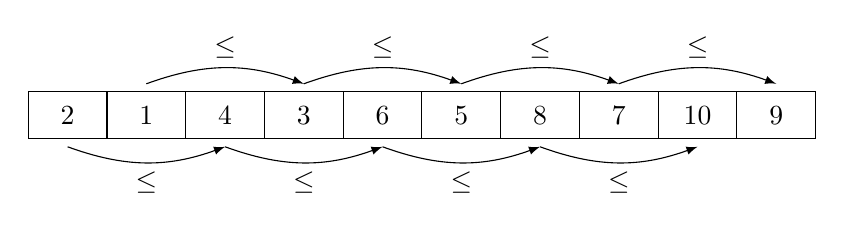
\begin{tikzpicture}[box/.style={rectangle, draw=black, minimum width=1cm,
                                minimum height=.6cm},]
\foreach \x/\y in {0/2, 1/1, 2/4, 3/3, 4/6, 5/5, 6/8, 7/7, 8/10, 9/9} {
  \node[box] at (\x,0){\y};
}

\foreach \i in {0, 2, 4, 6} {
  \draw[bend left=-20, -latex] (\i,-.4) to node[below]{$\le$} (\i + 2,-.4);
}

\foreach \i in {1, 3, 5, 7} {
  \draw[bend left=20, -latex] (\i,.4) to node[above]{$\le$} (\i + 2,.4);
}
\end{tikzpicture}
\end{center}

The \textsc{Merge-Lists-Min-Heap} algorithm (Question 6-5.9) can be used to
merge these $k$ subarrays in $O(n \lg k)$-time.

\item Item (e) shows that a $k$-sorted array has $k$ 1-sorted subarrays.  Note
that each of these subarrays must have at least $\floor{n / k}$ elements. Thus,
since $k$ is a constant, the lower bound to sort each of these subarrays is
\[
  \Omega\left(\frac{n}{k} \lg \frac{n}{k}\right) = \Omega\left(\frac{n}{k} \lg n - \frac{n}{k} \lg k\right) = \Omega(n \lg n),
\]
which implies that $\Omega(n \lg n)$ is also the lower bound to $k$-sort the
whole array.
\end{enumerate}
\end{framed}

\newpage

\item[8-6]{\textbf{\emph{Lower bound on merging sorted lists}}\\
The problem of merging two sorted lists arises frequently. We have seen
a procedure for it as the subroutine \textsc{Merge} in Section 2.3.1. In this
problem, we will prove a lower bound of $2n - 1$ on the worst-case number of
comparisons required to merge two sorted lists, each containing $n$ items.

First we will show a lower bound of $2n - o(n)$ comparisons by using a decision
tree,

\begin{enumerate}
\item[\textbf{a.}]{Given $2n$ numbers, compute the number of possible ways to
  divide them into two sorted lists, each with $n$ numbers.}
\item[\textbf{b.}]{Using a decision tree and your answer to part (a), show that
any algorithm that correctly merges two sorted lists must perform at least
$2n - o(n)$ comparisons.}
\end{enumerate}

Now we will show a slightly tigher $2n - 1$ bound.

\begin{enumerate}
\item[\textbf{c.}]{Show that if two elements are consecutive in the sorted order
and from different lists, then they must be compared.}
\item[\textbf{d.}]{Use your answer to the previous part to show a lower bound of
$2n - 1$ comparisons for merging two sorted lists.}
\end{enumerate}
}

\begin{framed}
\begin{enumerate}
\item Note that every list of elements only have one permutation that is in
sorted order. Thus, this problem can be seen as counting the number of ways to
pick $n$ numbers out of $2n$ numbers to form the first list, and using the
remaining numbers to form the second list. We can count that with the binomial
notation
\begin{equation*}
\begin{aligned}
  \binom{2n}{n} &= \frac{2^{2n}}{\sqrt{\pi n}} \left( 1 + O\left(\frac{1}{n}\right) \right),
\end{aligned}
\end{equation*}
in which the approximation is proved in (C.1-13).
\item The input of the merge algorithm are the two sorted lists and we know from
item (a) that the number of possible ways to form these lists elements is
$\binom{2n}{n}$. Note that these pairs of sorted lists are unique and each of
them can be the final merged list if placed side by side. Thus, the number of
permutations of the input to form the final merged list is also $\binom{2n}{n}$.
We can compute a lower bound on the number of comparisons to solve this problem
by determining the height of the decision tree with at least $\binom{2n}{n}$
leaves. Let $h$ be the height of such a decision tree. Thus, we have
\begin{equation*}
\begin{aligned}
  2^h &\ge \frac{2n}{n}\\
      &=   \frac{2^{2n}}{\sqrt{\pi n}} \left( 1 + O\left(\frac{1}{n}\right) \right),
\end{aligned}
\end{equation*}
which implies
\begin{equation*}
\begin{aligned}
  h &\ge \lg \left( \frac{2^{2n}}{\sqrt{\pi n}} \left(1 + O\left( \frac{1}{n} \right) \right) \right)\\
    &=   \lg (2^{2n}) - \lg(\sqrt{\pi n}) + \lg\left(1 + O\left( \frac{1}{n} \right)\right)\\
    &=   2n - o(n).
\end{aligned}
\end{equation*}

\item Let $A$ and $B$ denote the two input sorted lists and assume without loss
of generality that their elements are distinct. Let $a \in A$ and $b \in B$
denote two elements that are consecutive in the sorted order. Note that since
they are consecutive, the number of elements that are before/after $a$ in the
sorted list is equal to the number of elements before/after $b$ in the sorted
list. This implies that if we compare $a$ to every element of $B$ except $b$ and
compare $b$ to every element of $A$ except $a$, we will find the two possible
positions for them in the sorted list, but we will not be able to determine
which one comes first.

\item In the worst case, every pair of elements in the final list comes from
different input lists. There are $2n$ elements in the final list and $2n - 1$
pairs of consecutive elements. Thus, $2n - 1$ is a lower bound on the worst-case
number of comparisons to merge two sorted lists.
\end{enumerate}
\end{framed}

\newpage

\item[8-7]{\textbf{\emph{The 0-1 sorting lemma and columnsort}}\\
\emph{Very long statement. Read it on the text book.}
}

\begin{framed}
Skipped.
\end{framed}

\end{enumerate}

\end{document}
